\documentclass[10pt,fleqn]{article} % Default font size and left-justified equations
\usepackage{import}
\usepackage[%
    pdftitle={Energie et puissance d'un smartphone},
    pdfauthor={Geoffrey Vaquette}]{hyperref}
\subimport{../../../../style/}{preambule}
%\fichetrue
\fichefalse

\proftrue
%\proffalse

\tdtrue
%\tdfalse

\courstrue
%\coursfalse

\subimport{../../../../style/}{new_style}
\subimport{../../../../style/}{macros_SII}
\subimport{../../../../style/}{preambule_trou}

\usepackage{siunitx}
% -------------------------------------
% Déclaration des titres
% -------------------------------------

\def\discipline{Enseignement \\Technologique \\ Transversal}
\def\xxtete{Enseignement Technologique Transversal}

\def\classe{1 STI2D}
\def\xxnumpartie{Séquence 2}
\def\xxpartie{Energie électrique et puissance d'un smartphone}

\def\xxnumchapitre{Séance 3}
\def\xxchapitre{\hspace{.12cm} Énergies, Puissances et rendement}

\def\xxposongletx{2}
\def\xxposonglettext{1.45}
\def\xxposonglety{23}
\def\xxonglet{Seq. 2 -- TD 3}

\def\xxactivite{TD}
\def\xxauteur{\textsl{Geoffrey Vaquette}}

\def\xxcompetences{%
\textsl{%
\textbf{Savoirs et compétences :}
\begin{itemize}[label=\ding{112},font=\color{ocre}]
\item CO2.1	Identifier les flux et la forme de l'énergie, caractériser ses transformations et/ou modulations et estimer l'efficacité globale d'un système.
\end{itemize}
%
}}

\def\xxfigures{
\begin{center}
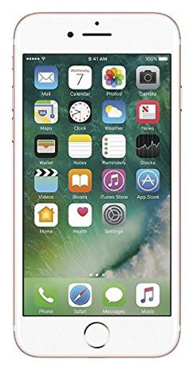
\includegraphics[height=4cm]{images/smartphone.png} \\
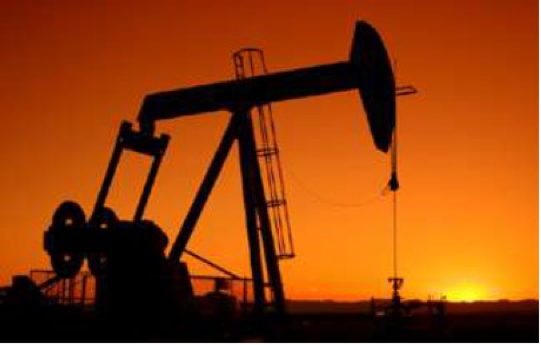
\includegraphics[height=4cm]{images/petrole.png} \\
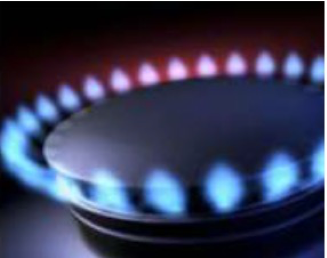
\includegraphics[height=4cm]{images/gaz.png} \\
\end{center}
}%figues de la page de garde
\def\xxpied{%
Energies, Puissances et Rendement \xxactivite%
}

%---------------------------------------------------------------------------

\renewcommand{\RemplirTrou}{true}
\begin{document}
\chapterimage{png/Fond_solaire}

\begin{obj}
Déterminer l’énergie et la puissance disponibles dans un système

L’étude suivante concerne un BlackBerry Bold 9780 à travers laquelle vous serez amené à
 calculer l’énergie présente dans la batterie de ce téléphone ainsi que les puissances 
 nécessaires pour différentes utilisations de celui-ci.
 
\end{obj}
\section{Étude énergétique d'un ancien smartphone}
\subsection{Quelques données}
Caractéristiques de la batterie :
\begin{itemize}
 \item Technologie : Li-Ion (lithium-ion)
\item Capacité : $ C = \SI{1500}{mAh} $
\item Tension : $U=\SI{3.7}{V}$
\item Autonomie en conversation : jusqu'à 6 heures
\item Autonomie en veille : jusqu’à 528 heures
\item Autonomie en lecture de musique : jusqu'à 36 heures
\end{itemize}



\begin{exercise}~

\begin{question}
  Quelle solution permet de remplir la fonction « Alimenter / Stocker » ?
\end{question} 
\begin{solution}
  La fonction alimenter/stocker est réalisée par la batterie du smartphone. 
\end{solution}

\begin{question}
  Calculer l’énergie électrique $\omega_\text{bat}$que contient la batterie.
\end{question}
\begin{solution}
  On connaît la tension de la batterie, ainsi que sa capacité. L'énergie 
  contenue dans la batterie est $$\omega_text{bat} = U\times C = 1.5\times 3.7 =\SI{5.5}{Wh} $$
\end{solution}

\begin{question}
  A partir des données annoncées, calculer la puissance de ce Smartphone en 
  conversation, en veille et en lecture de musique. 
\end{question}
\begin{solution}
$$P = \frac{\omega_text{bat}}{t}
P_{\text{conv}} = \frac{5,55}{6} = \SI{0.925}{W}
P_{\text{veille}} = \frac{5,55}{\num{528e-3}} = \SI{10.5}{mW}
P_{\text{musique}} = \frac{5,55}{\num{36e-3}} = \SI{154.2}{mW}$$
\end{solution}

\begin{question}
  En déduire le courant consommé en conversation, en veille et en lecture de musique.
\end{question}
\begin{solution}
  Connaissant la relation liant la puissance, le courant et la tension 
  $P=U\times I$, on déduit $I = \frac{P}{U}$
  $$
 I_{\text{conv}} = \frac{0,925}{3,27} = \SI{283}{mA}
  I_{\text{veille}} = \frac{10.5}{3,27} = \SI{3.21}{mA}
   I_{\text{musique}} = \frac{0.1542}{3,27} = \SI{47}{mA}$$
\end{solution}

\begin{question}
  En supposant qu’une charge complète de la batterie doit être effectuée tous les 6 jours, déterminer l’énergie électrique consommée en une année.
\end{question}
\begin{solution}
  Tous les 6 jours, le Smartphone consomme une énergie de 5,55 Wh.
Il faudra donc le recharger 61 fois en un an (nb = 365 / 6 = 61).
Wannuelle = 61 x 5,55 = 335,5 Wh
\end{solution}

Les questions précédentes utilisent des données d'un smartphone des années 2000. 
Aujourd'hui, prenons l'exemple du \textit{Samsung Galaxy S9} dont quelques 
caractéristiques sont données ci-dessous. 

\begin{itemize}
  \item Capacité de la batterie : $C_{S9} = \SI{3000}{mAh}$
  \item Tension de la batterie : $U_{S9} = \SI{4.4}{V}$
  \item Autonomie mesurée en utilisation : $A = \SI{11}{h} et \SI{20}{min}$
\end{itemize}
\begin{question}
  Calculez l'énergie de la batterie et comparez-la avec celle du précédent 
  smartphone.
\end{question}
\begin{solution}
  $$\omega_\text{S9} = 11.33 \times 3000 = \SI{33990}{mWh}$$
  Elle est plus de 6 fois supérieure à celle d'un ancien modèle
\end{solution}

\begin{question}
  Calculez la puissance en utilisation de ce smartphone.
\end{question}

\begin{question}
  En supposant une recharge tous les 2 jours, estimez l'énergie consommée sur 
  une année. Concluez. 
\end{question}
\end{exercise}


\end{document}